% tex file for convolution
\subsubsection{Convolution}
\par \indent Our study is structured around event-related neurological 
stimuli, rather than block stimuli as was the case of the data used in 
class examples. So, we could not repurpose the class approach for 
representing the hemodynamic response to our analysis. 

\par It is assumed that there is a relationship between the hemodynamic 
response to the neurological stimuli. Further, there is the assumption that 
a single stimulus generates a delayed hemodynamic response that mirrors a 
double-gamma function, and that multiple stimuli have an additive nature, as 
defined below: 

\begin{equation} \label{eq:convolve}
r(t)= \sum_{i=1}^n \psi_{i} \phi_{i}(t-t_i)
\end{equation}

\noindent where $\psi_i$ is the amplitude of the response stimulus (assumed to 
be always $1$ in our case), and $\phi_{i}$ is the hemodynamic response started 
at the $i$th stimulation ($t_i$).

\par We attempted five approaches that can each be grouped into one of three 
subcategories: \textbf{(1)} a strict replication of equation 
\ref{eq:convolve}; \textbf{(2)} a matrix multiplication equivalent to 
\textbf{(1)}; and \textbf{(3)} a complex function that takes advantage of the 
speed of \texttt{np.convolve}. This complicated function \textbf{(3)} first 
splits the (two-second) intervals between each scan into a given number of 
even slices, then puts the stimulus into the closest slice with respect to 
time, and finally calls \texttt{np.convolve} on this much longer time series 
and a detailed hrf function, before reducing it back down to the dimensions of 
the original scan time series at two-second intervals. Detailed exploration of 
this matter can be found in Appendix \ref{app_convolution}.

We compared these methods for on accuracy and speed. Figure 
\ref{fig:convolution_a} displays an accuracy comparison, and Table 
\ref{tab:convolution_a} shows the speed per loop based off of 
\texttt{iPython}'s \%\texttt{timeit} magic command.



\begin{figure}[ht]
\centering
\begin{minipage}[b]{0.45\linewidth}
	\centering
	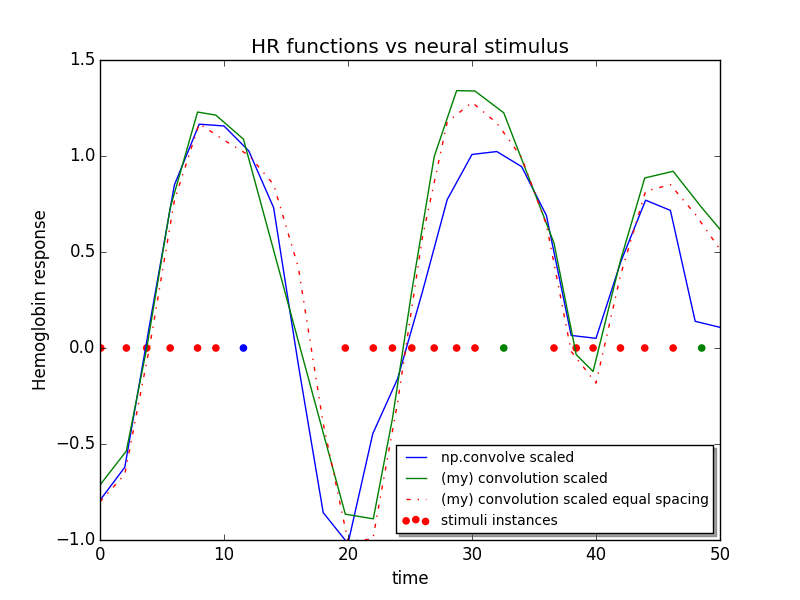
\includegraphics[width=.8\linewidth]{../images/convolution_vs_neural_stimulus}
	% needs to be from the event_related_HRF_script2.py 
	\caption{\scriptsize{Different convolution functions vs. 
the Neural stimulus}}
	\label{fig:convolution_a}

\end{minipage}
\quad
\begin{minipage}[b]{0.45\linewidth}
	\centering
	\begin{tabular}{|l | c|}
	\hline
	name in graph       & Speed per loop \\
	\hline
	np naive approach & 14.4 $\mu$s  \\
	user 2     		    & 972 ms  \\
	user 3     		    & 1.15 s    \\
	user 4 (15 cuts)      & 98.3 ms \\
	user 4 (30 cuts)      & 185 ms  \\
	user 5     	 	    & 110 ms   \\
	\hline
	\end{tabular}
	\vspace{5mm}
\captionof{table}{\scriptsize{Speed to create HRF predictions for 
	Subject 001, all conditions}}
	\label{tab:convolution_a}
	\end{minipage}
\end{figure}

\par \noindent The first method in the table, ``np naive approach'', blindly 
plugs our data into the \texttt{np.convolve} function. This approach is 
ill-advised, because our data fails the \texttt{np.convolve} assumption of 
equidistant spacing for stimuli and scans. It is only demonstrated to showcase 
potential speed. The failure of the ``np naive approach'' was the motivating 
factor behind the rest of the hemodynamic response convolution analysis. The 
``user 2'' and ``user 3'' functions fall under subcategory \textbf{(1)}. 
``user 2'' was the first approach designed to approximate the theoretical 
background, but it matches the stimulation times and not the scan times.
``user 3'' is the most theoretically sound model (and is our standard for 
accuracy). ``user 5'' falls under subcategory \textbf{(2)} and is the matrix 
algebra version ``user 3'', with identical accuracy and gains in speed. 
``user 4'' falls under subcategory \textbf{(3)}, the methods that use the
grid cut usage of \texttt{np.convolve} with notations for the number of slices 
between each scan. We concluded that "user 4 (15 cuts)" was the best approach 
since it gives us much more speed and very close accuracy to the golden 
standard --- ``user 3''.

\subsubsection{Time Correction}

\par \indent The fMRI scanner scans each voxel at a slightly different time. 
In our case, the lowest horizontal slice was scanned first, with the later 
scans obtained progressively in order toward the top of the brain. The signs 
of this linear change in time of scan were observed when we ran simple linear 
regression on the data and found that the hemodynamic response $\hat{\beta}$ 
values from all conditions were grouped together. We corrected for the time 
differences by shifting the times of stimuli ``backwards'' for voxels scanned 
later to directly correct for the delay of the scan (assuming that each layer 
of the scan took 2/34 of a second).

\subsubsection{Multiple Conditions}

\par \indent Originally, we tried using multiple linear regression to account 
for the three different types of stimuli (pump, explode, cash-out) and 
examined if the separation of these stimuli can better describe the response. 
We did this by creating separate predicted hemodynamic responses for each 
condition to allow for different amplitudes associated with each type of 
condition. As will be noted in Section \ref{model_selection} later, we did 
not observe a large difference in the results values we obtained from 
predicting the hemodynamic responses together for all conditions, so we did 
not continue with this exploration. In Figure \ref{fig:all_cond_time}, we can 
see the different conditions separated the responses for each condition.
 

\begin{figure}[ht]
\centering
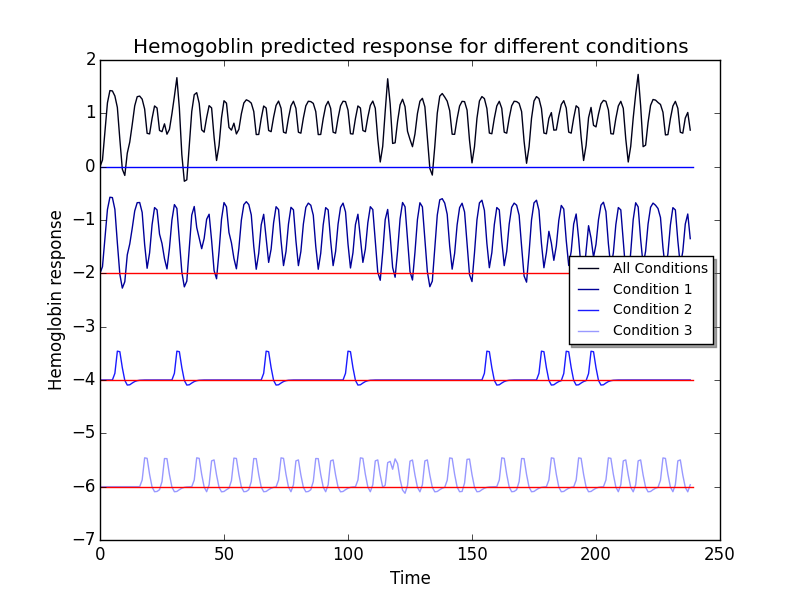
\includegraphics[scale=.5]{../images/all_cond_time}  
\caption{Plotting all predicted HR for conditions.}
\label{fig:all_cond_time}
\end{figure}

\par A more detailed discussion about our approach and the theory behind the 
convolution of the hemodynamic response with the neurological response 
can be found in Appendix \ref{app_convolution}.

